The performance evaluation is split into two: a shared memory performance
scaling evaluation on a 64 core machine, and a distributed memory performance
evaluation on a cluster on up to 12 nodes.

\subsection{Evaluation Methodology}

The performance evaluation aimed to test the scalability of the parallelised
application in two ways. The first is with a fixed area under test. This will
show how a given problem (150x150x90 in size) would scale to larger machines and
in a cluster. The second test is with an expanding area. This is where, for all
runs, each process has its own area of a set size (150x150x90) such that, as the
number of processes grows, the overall computational area increases at the same
rate. This will show well larger problem sets can be handled and how the
overhead of communication grows as the number of processes involved in the
communication grows.

For a given number of processes, there can be many runs. This is because the
layout of processes matters. For instance, the 64 process runs are executed in a
4x16, 8x8, and 16x4 layout. The quickest layout is reported as the runtime for
that number of processes.

\subsection{Shared-memory parallelisation}

The shared-memory parallelisation run was conducted on a machine called togian.
This system is a quad socket AMD Opteron 6366HE system giving it 64 cores paired
into 32 modules running at 1.8GHz. To provide consistent benchmarking results,
the turbo clock frequencies were disabled. The system has been fitted with 512GB
of DDR3 RAM.

\subsubsection{Default Mapping}

The first configuration under evaluation was the default setup for MPICH 3.1.3.
This default mapping assigns processes to cores in a round-robin fashion across
sockets. This spreads the runtime load between CPU sockets thus minimising the
load on the CPUs cache for small numbers of processes and maximises the chance
of achieving a higher turbo clock frequency if applicable.

\begin{figure}
    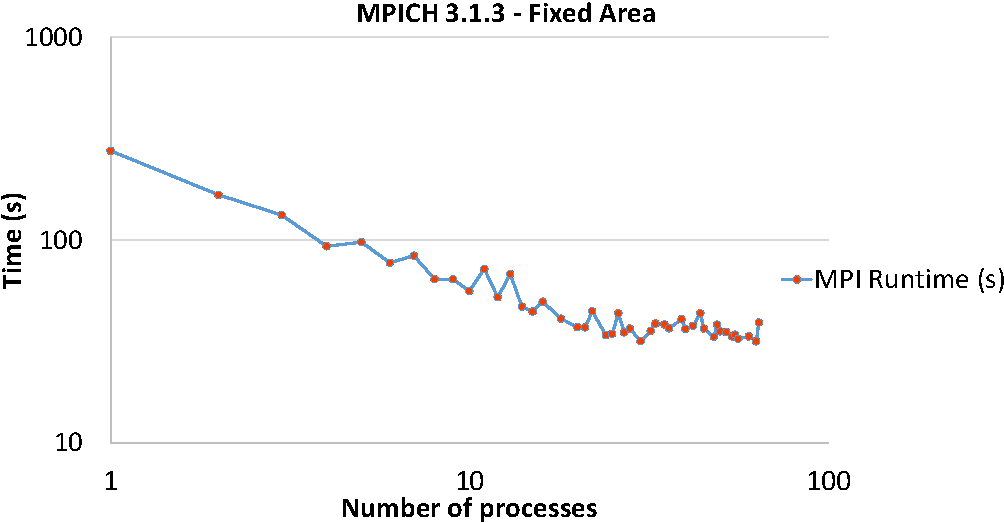
\includegraphics[page=1,width=0.5\textwidth]
    {graphs/MPICH313-default-mapping-fixed-area-crop.pdf}
    \caption{MPICH 3.1.3 Default Mapping Fixed Area}
    \label{fig:mpichdefaultmappingfixedarea}
\end{figure}

Figure~\ref{fig:mpichdefaultmappingfixedarea} shows linear improvements in
runtime for a fixed sized area. Single threaded performance brings runtime to
275.5 seconds with 64 threads completing its run in 39.2 seconds, a 7x
improvement in computational throughput.

The graph isn't as smooth as would normally be expected. This is as a direct
consequence to the mapping of processes over a two dimensional area. If the same
number of processes exist in both axes, then the performance is at its best
since the length of all halos are equal. In an extreme case, the runs that have
a prime number of processes (11 and 13 for instance) by definition cannot have a
balanced layout thus two halos will be significantly shorter than the others.
This difference acts as a bottleneck since the shorter halo exchanges finish
sooner then have to wait for the longer halo exchanges to complete.

\begin{figure}
    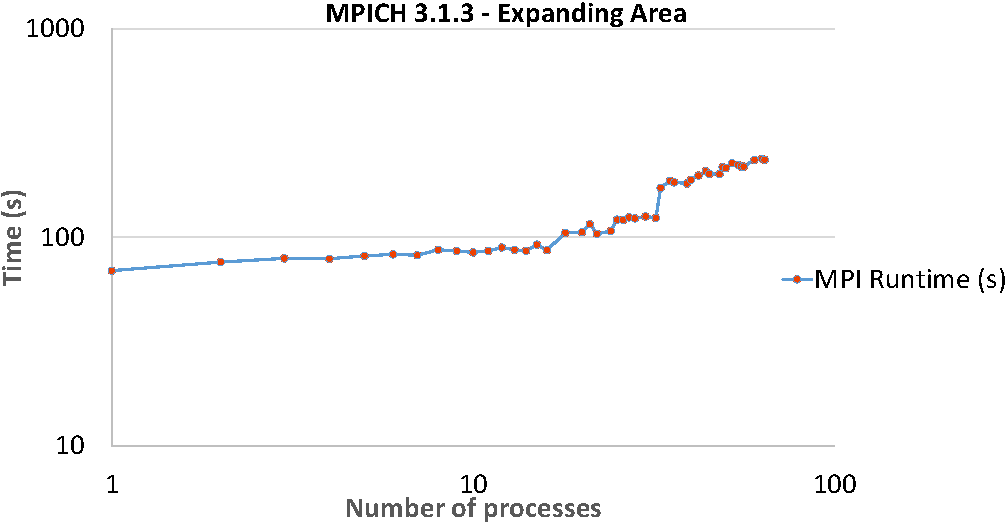
\includegraphics[page=1,width=0.5\textwidth]
    {graphs/MPICH313-default-mapping-expanding-area-crop.pdf}
    \caption{MPICH 3.1.3 Default Mapping Expanding Area}
    \label{fig:mpichdefaultmappingexpandingarea}
\end{figure}

Figure~\ref{fig:mpichdefaultmappingexpandingarea} shows good scaling of runtime
where the overall area under simulation grows at the same rate as the process
count. A single process executing on a 150x150x90 area takes 69.2 seconds to
execute whereas 64 processes executing on a 1200x1200x90 area takes 235.9
seconds to execute. This equates to a 3.4x increase in runtime for a 64x
increase in area, improving throughput by 18.8x. Comparing this with the fixed
area improvement of 7x, it is clear to see that to get the most benefit from the
MPI parallelised LES is to calculate velocities over greater areas or at greater
resolutions than before. This is also as intuition would expect since the setup
cost of sending a message is fixed irrespective of the message size so larger
messages amortize the cost of the setup. Also, as the fixed area runs gain
processes, the ratio between useful computation and message sending decreases.

Towards the end of the graph there is a significant increase. This occurs on the
move from 32 to 33 processes. This is because at 32 processes, all sockets are
exactly `half full'. Each module has its own hardware thread active so each
process has its own floating point units. On the move to 33 processes, a process
will now have to share floating point units with another process. This will slow
down these processes and, by extension, the application overall. This is a
feature of the AMD CPU architecture and not something caused by MPI or the LES.

\subsubsection{By Core Mapping}

The second configuration under evaluation involved a minor change to MPICH
3.1.3. Instead of using the default mapping of processes to cores, mpiexec was
setup to assign processes to cores sequentially. This means a single socket will
be `filled up' with processes before moving on to the next. The rationale behind
this change was to increase the probability that a processes neighbours were on
the same socket. This is almost always now true for the left and right neighbour
which will be running on the previous and next core respectively. The primary
downsides are increased cache and floating point unit utilisation on smaller
process counts. For example, a four process run is now sharing the resources of
a single socket rather than each having the resources of their own socket.
Another downside is that the turbo frequency will be reduced quicker on
applicable systems since a socket will reach higher process counts sooner.

\begin{figure}
    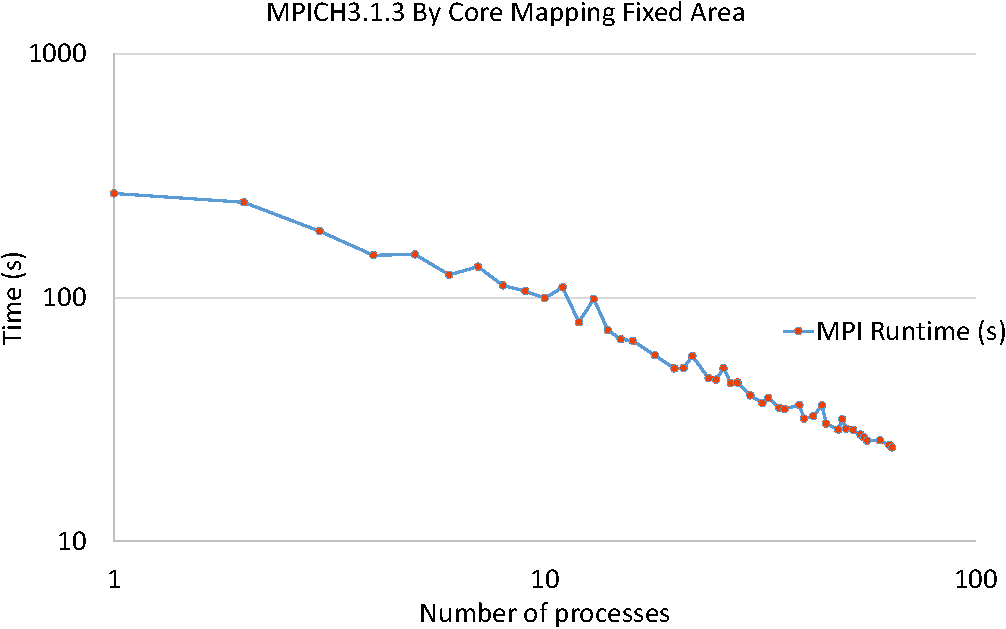
\includegraphics[page=1,width=0.5\textwidth]
    {graphs/MPICH313-by-core-mapping-fixed-area-crop.pdf}
    \caption{MPICH 3.1.3 By Core Mapping Fixed Area}
    \label{fig:mpichbycoremappingfixedarea}
\end{figure}

Figure~\ref{fig:mpichbycoremappingfixedarea} shows that, for the fixed area
runs, the performance difference is negligible. The lower process counts have
poorer performance however, once the 32 process boundary has been crossed,
performance is the same as the default mapping case.

\begin{figure}
    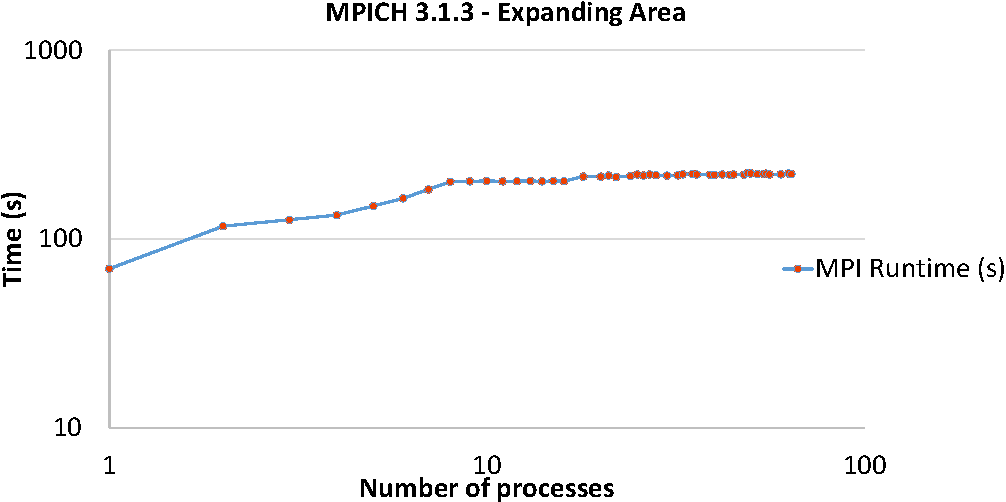
\includegraphics[page=1,width=0.5\textwidth]
    {graphs/MPICH313-by-core-mapping-expanding-area-crop.pdf}
    \caption{MPICH 3.1.3 By Core Mapping Expanding Area}
    \label{fig:mpichbycoremappingexpandingarea}
\end{figure}

Figure~\ref{fig:mpichbycoremappingexpandingarea} again shows good scaling of
runtime where the overall simulation area increases at the same rate as the
process count increases. It also shows more clearly that runtime levels out so
increases in area are `for free' when increasing the process count by the same
amount. Runtime now levels out at around 220 seconds which is a 7\% improvement
over the default mapping case. This change isn't massive but is consistent and
shows that tweaks outside of the code itself can benefit performance.

As expected, the performance at small process counts is significantly poorer
than in the default mapping case.

\subsubsection{MPICH versus OpenMPI}

\begin{figure}
    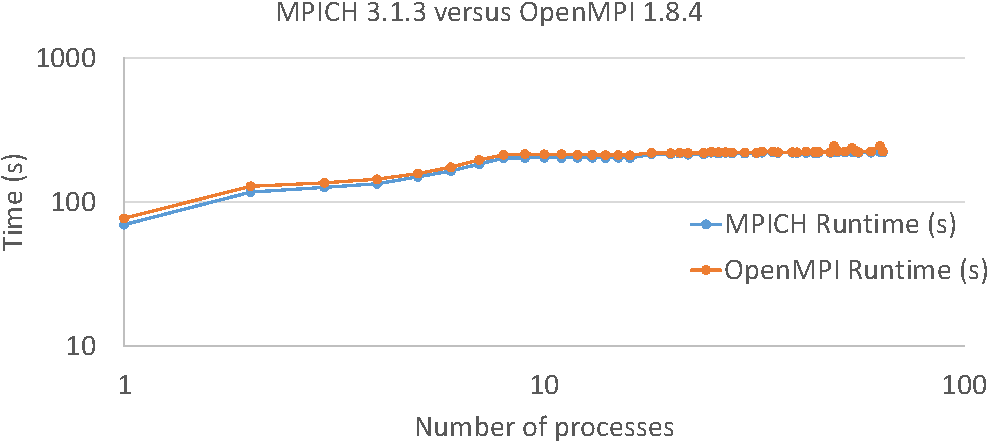
\includegraphics[page=1,width=0.5\textwidth]
    {graphs/MPICH313-versus-OpenMPI184-crop.pdf}
    \caption{MPICH 3.1.3 Versus OpenMPI 1.8.4 Expanding Area}
    \label{fig:mpichversusopenmpiexpandingarea}
\end{figure}

Figure~\ref{fig:mpichversusopenmpiexpandingarea} shows how there is no tangible
performance difference between MPICH 3.1.3 and OpenMPI 1.8.4.

\subsection{Distributed-memory paralellism}

Results were obtained using the EPSRC funded ARCHIE-WeSt High Performance
Computer (\url{www.archie-west.ac.uk}). EPSRC grant no. EP/K000586/1.

Each node has two Intel Xeon X5650 CPUs. 12 cores running at 2.66GHz (with
turbo). 48GB RAM 4xQDR Infiniband Interconnect

\begin{figure}
    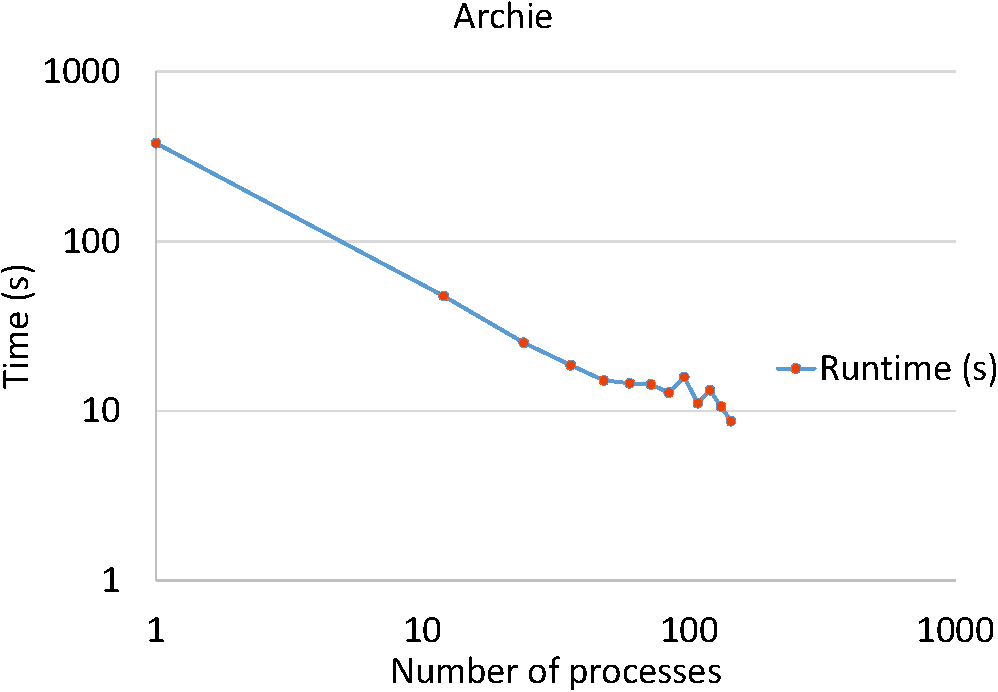
\includegraphics[page=1,width=0.5\textwidth]
    {graphs/ARCHIE-OpenMPI162-GFORTRAN482-default-mapping-fixed-area-crop.pdf}
    \caption{ARCHIE Fixed Area}
    \label{fig:archiefixedarea}
\end{figure}

\begin{figure}
    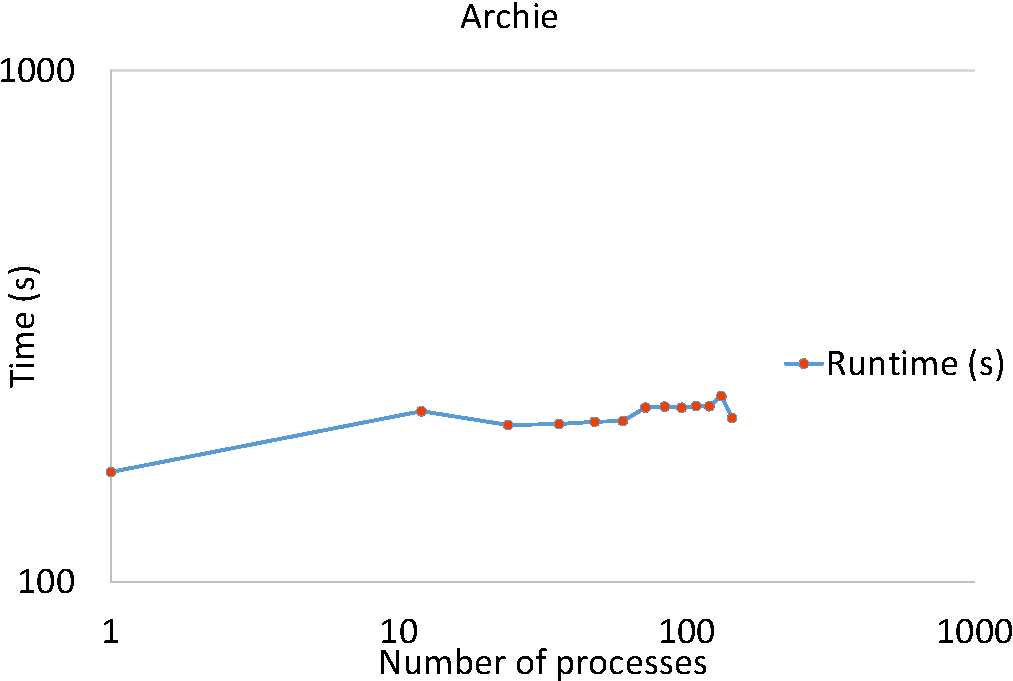
\includegraphics[page=1,width=0.5\textwidth]
    {graphs/ARCHIE-OpenMPI162-GFORTRAN482-default-mapping-expanding-area-crop.pdf}
    \caption{ARCHIE Expanding Area}
    \label{fig:archieexpandingarea}
\end{figure}

\subsection{Estimated versus exact corners}

The majority of the communication in the LES involves halo exchanges. These
involve sending and receiving up to four edges between neighbouring processes.
To be mathematically correct, there would also need to be up to four other
communications, a small number of values need to be sent and received for corner
values from four other processes. This brings the total number of messages per
process up to eight. This was thought to be a potential source of overhead,
especially given the overhead of sending a single message was likely to outweigh
the transfers itself. To test this, all runs were reran with corners instead
being calculated rather than exchanged.

For the shared memory runs, there was a negligible change in performance. This
is likely to be because the cost of calculating floating point units is very
similar to simple memory copies between memory spaces, especially in an AMD
system where floating point units are shared between pairs of cores in what AMD
calls a module.

For the distributed memory runs, exact corners were up to 5\% faster than the
estimated corner runs. The improvement is somewhat more surprising than the
shared memory case however given the fast Infiniband Interconnect between nodes,
the cost of sending a message is likely to be only marginally higher than
communication within a single node. The performance improvement is likely due to
the Xeon X5650's older architecture meaning it supports fewer instruction set
extensions such as AVX and FMA that are known to improve integer and floating
point operation performance.
